\documentclass{report}
\usepackage[T1]{fontenc} % Fontes T1
\usepackage[utf8]{inputenc} % Input UTF8
\usepackage[backend=biber, style=ieee]{biblatex} % para usar bibliografia
\usepackage{csquotes}
\usepackage[portuguese]{babel} %Usar língua portuguesa
\usepackage{blindtext} % Gerar texto automaticamente
\usepackage[printonlyused]{acronym}
\usepackage{hyperref} % para autoref
\usepackage{graphicx}
\usepackage{subcaption}


\bibliography{bibliografia}


\begin{document}
%%
% Definições
%
\def\titulo{TRABALHO DE APROUNDAMENTO 2}
\def\data{9/05/2020}
\def\autores{Rafael Santos-98466, Hugo Domingos-98502}
\def\autorescontactos{}
\def\versao{}
\def\departamento{DEPARTAMENTO DE ELTRÓNICA,TELECOMUNICAÇÕES E INFORMÁTICA}
\def\empresa{}
\def\logotipo{download.jpeg}
%
%%%%%% CAPA %%%%%%
%
\begin{titlepage}

\begin{center}
%
\vspace*{50mm}
%
{\Huge \titulo}\\ 
%
\vspace{10mm}
%

%
\vspace{10mm}
%
{\LARGE \autores}\\ 
%
\vspace{30mm}
%
\begin{figure}[h]
\center
\includegraphics{\logotipo}
\end{figure}
%
\vspace{30mm}
\end{center}
%
\begin{flushright}
\versao
\end{flushright}
\end{titlepage}

%%  Página de Título %%
\title{%
{\Huge\textbf{\titulo}}\\
{\Large \departamento\\ \empresa}
}
%
\author{%
    \autores \\
    \autorescontactos
}
%
\date{\data}
%
\maketitle

\pagenumbering{roman}

\tableofcontents
% \listoftables     % descomentar se necessário
% \listoffigures    % descomentar se necessário


%%%%%%%%%%%%%%%%%%%%%%%%%%%%%%%
\clearpage
\pagenumbering{arabic}

%%%%%%%%%%%%%%%%%%%%%%%%%%%%%%%%
\chapter{Introdução}
\label{chap.introducao}

Este trabalho de aprofundamento foi-nos proposto no âmbito da unidade curricular de Laborátorios de Informática.

Este projeto trata-se de um processo de ordenação de várias pessoas que participam num certo evento. Cada um vai obter aleatoriamente um número de ordem .

Quando cada um revelar o seu número de ordem todos poderão comprovar que não há números coincidente. 

\chapter{Metodologia}
\label{chap.metodologia}
Neste projeto, tal como aconselhado pelos docentes da unidade curricular, foram usados sockets TCP para a comunicação entre o servidor e o cliente,sendo também usado o código fornecido pelos docentes tal como b64.py , common\_com.py ,e cifradecifra.py.
\indent Para realizar este projeto foram usados os conhecimentos de sockets,de criptografia e de ficheiros CSV.
\pagebreak
\section{Comunicação Servidor-Cliente}
\subsection{Servidor}
Partindo do código inicial fornecido pelos professores, foi-nos necessário numa fase inicial colocar o servidor a funcionar.

\begin{figure}[hbt!]
  \centering
  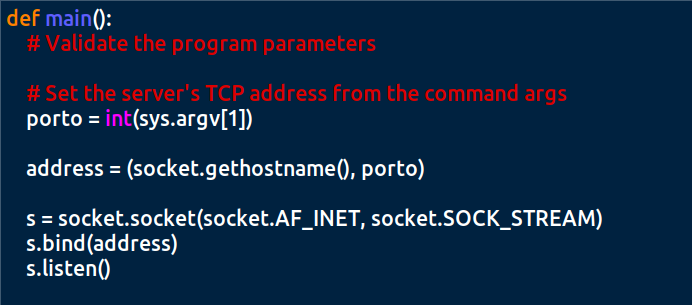
\includegraphics[width=1\linewidth]{MainServer.png}
  \caption{Inicialização do Servidor}
\end{figure}
Na figura 2.1, no que respeita ao "porto",este é definido através da consola e serve para nomear a socket.O parametro "s" é relativo à criação da socket TCP.É utilizado o bind associado à socket "s" para que seja definido o "end point" da comunicação;
\pagebreak
\subsection{Cliente}
Com o servidor ativo foi necessário conectar o cliente ao servidor, sendo necessário colocar os parametros na consola.

\begin{figure}[hbt!]
  \centering
  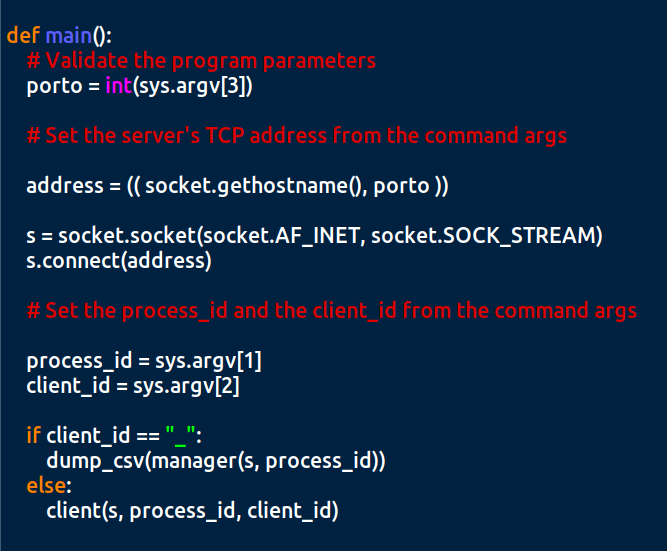
\includegraphics[width=1\linewidth]{cliente.png}
  \caption{Cliente}
\end{figure}
Para que o cliente entre em contacto com o servidor é necessário recorrer às informações atribuidas ao servidor, tal como o "address" e o "porto".\newline
Para iniciar o cliente é necessário colocar o id do processo(process\_id) e o id do cliente(client\_id), aquilo que vai identificar o participante.\newline
\indent Se o id for "\_" , vai ser gerado o processo onde poderemos aceder ao número e identidade dos participantes e realizar o processo de distribuição.
\pagebreak
Caso seja tentado adicionar um participante mas o cliente ainda não tenha sido criado, irá ser impresso no ecrã :"Server error: Sorting process no found".
Se for tentado ser criado um novo processo com mesmo novo do já criado o erro será: "error':'Sorting process already exists ".
Caso o participante 1 tenha o mesmo id que o participante 2 deverá ocorrer : "'error':'Client already registered in sorting process' ".

\begin{figure}[h!]
\centering
\begin{subfigure}{.5\textwidth}
  \centering
  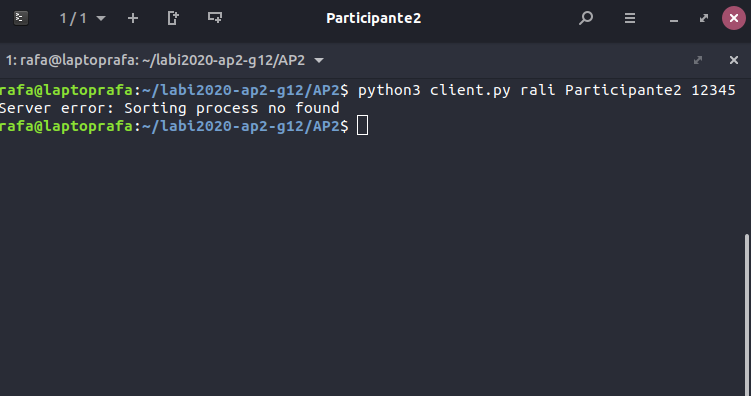
\includegraphics[width=0.9\linewidth]{erroP.png}
  \caption{Sorting process not found}
\end{subfigure}%
\begin{subfigure}{.5\textwidth}
  \centering
  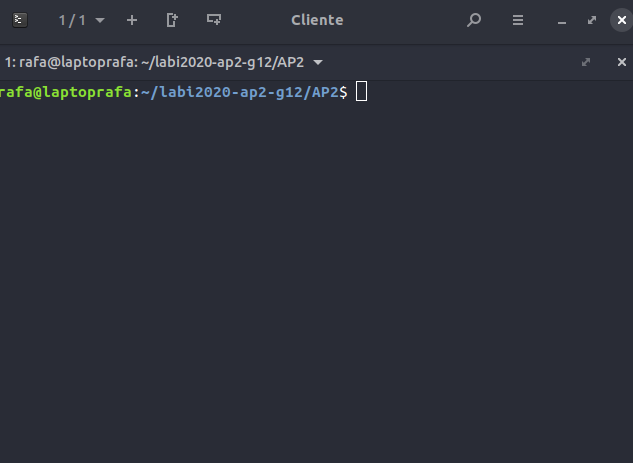
\includegraphics[width=0.9\linewidth]{ClientNaoCriado.png}
  \caption{Cliente não criado}
\end{subfigure}
\begin{subfigure}{.5\textwidth}
  \centering
  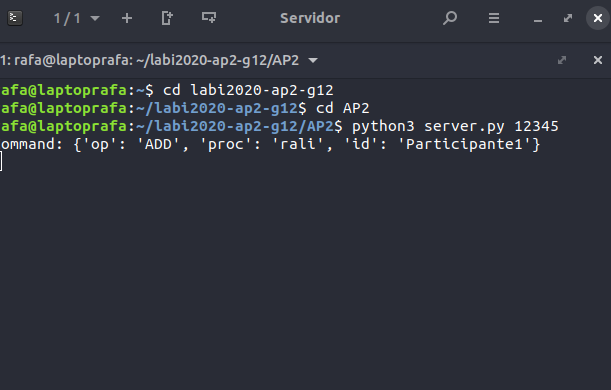
\includegraphics[width=0.9\linewidth]{server2.png}
  \caption{Servidor ativo}
\end{subfigure}%
	\caption{Sorting process not found}
\end{figure}

\begin{figure}[h!]
\centering
\begin{subfigure}{.5\textwidth}
  \centering
  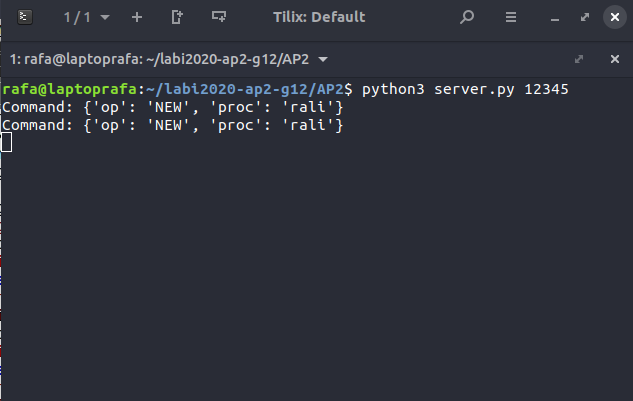
\includegraphics[width=0.9\linewidth]{ServerAtivo.png}
  \caption{Servidor ativo}
\end{subfigure}%
\begin{subfigure}{.5\textwidth}
  \centering
  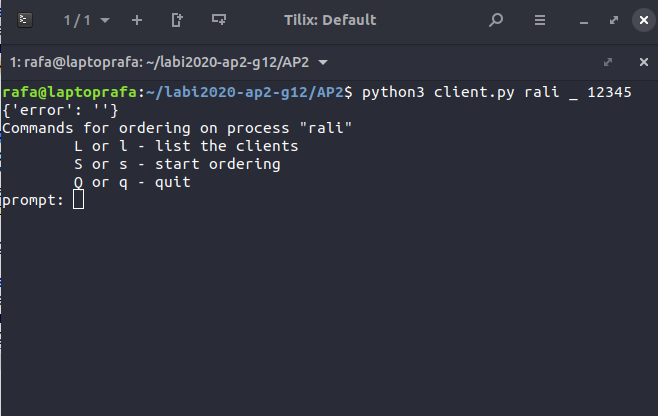
\includegraphics[width=0.9\linewidth]{Sorting.png}
  \caption{Processo de sorting criado}
\end{subfigure}
\begin{subfigure}{.5\textwidth}
  \centering
  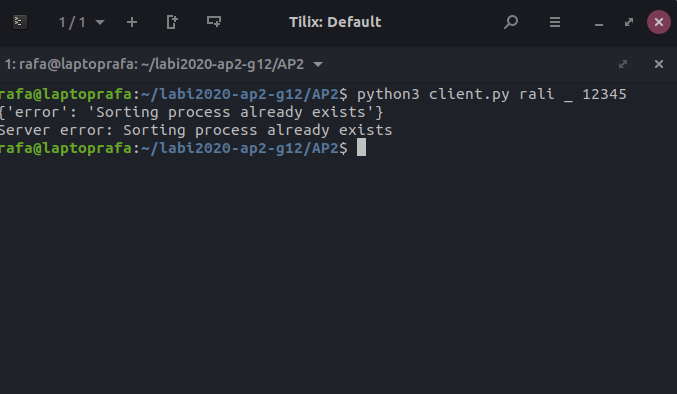
\includegraphics[width=0.9\linewidth]{SortingAlreadyExists.png}
  \caption{error:Sorting process already exists}
\end{subfigure}%
	\caption{Sorting process not found}
\end{figure}
\paragraph{}

\begin{figure}[h!]
\centering
\begin{subfigure}{.5\textwidth}
  \centering
  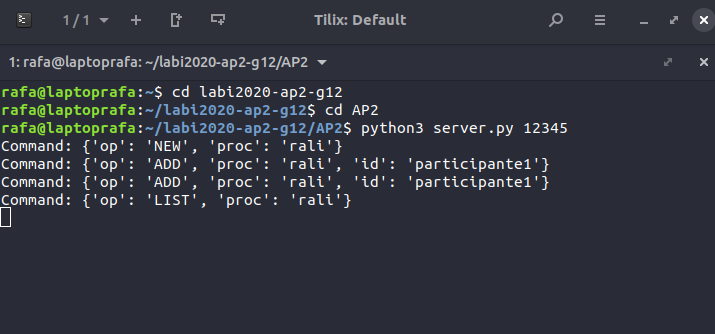
\includegraphics[width=0.9\linewidth]{ServidorAtivo.png}
  \caption{Servidor ativo}
\end{subfigure}%
\begin{subfigure}{.5\textwidth}
  \centering
  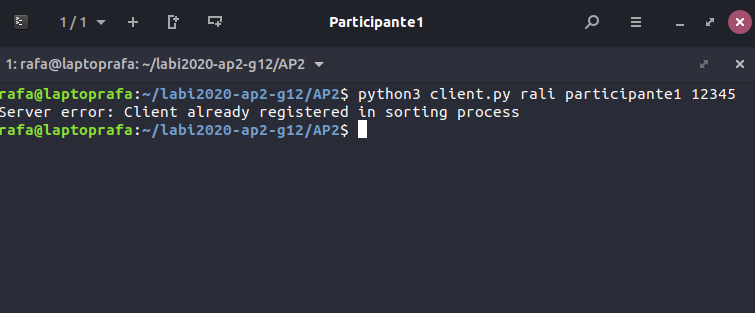
\includegraphics[width=0.9\linewidth]{erroCliente.png}
  \caption{error:Client already registered in sorting process}
\end{subfigure}
\begin{subfigure}{.5\textwidth}
  \centering
  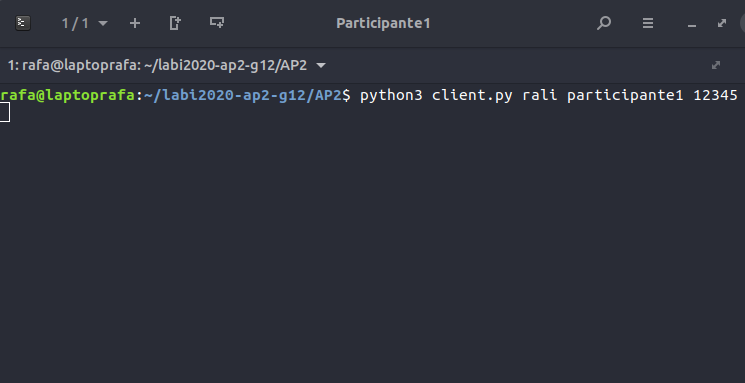
\includegraphics[width=0.9\linewidth]{ParticipanteJaCriado.png}
  \caption{Participante1 já criado}
\end{subfigure}%
	\caption{error:Client already registered in sorting process}
\end{figure}


\pagebreak
\paragraph{}

\subsection{Processo de distribuição}
	Feita a conexão entre o servidor e o cliente é necessário colocar os participantes no processo.Iremos chamar ao processo "rali".
	O utilizador terá a opção de listar os clientes e inicializar o processo de ordenação.
	\paragraph{}
\begin{figure}[hbt!]
  \centering
  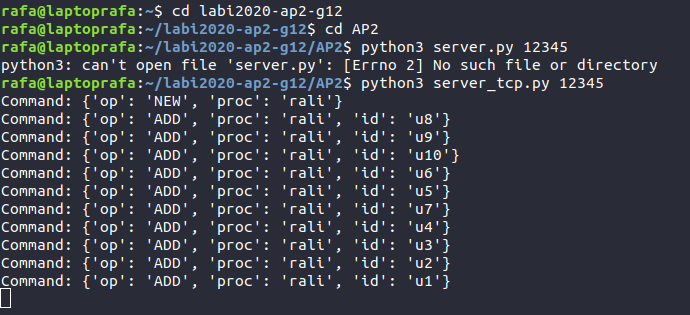
\includegraphics[width=0.9\linewidth]{ServerComPart.png}
  \caption{Servidor com 10 participantes já listados .}
\end{figure}

\begin{figure}[hbt!]
  \centering
  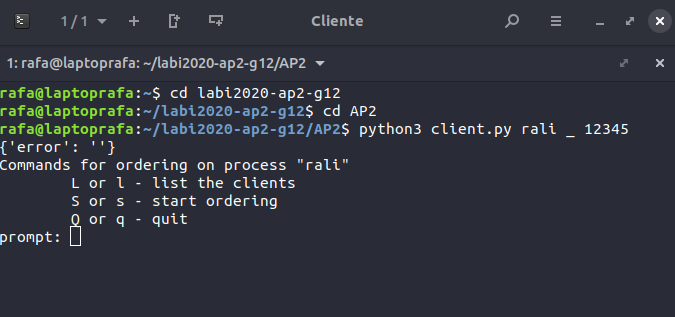
\includegraphics[width=0.9\linewidth]{clienteConsola.png}
  \caption{Cliente}
\end{figure}

	

\chapter{Resultados}
\subsection{Listagem dos clientes}
Olhando para o cliente, ao pressionar-mos "l" obtemos a identificação dos participantes por ordem de entrada no processo "rali".
\begin{figure}[hbt!]
  \centering
  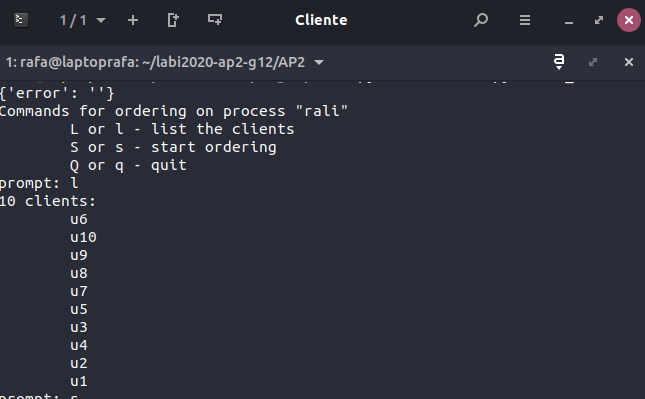
\includegraphics[width=0.7\linewidth]{ListaParticipantes.png}
  \caption{Participantes ordenados por ordem de entrada no processo.}
\end{figure}*
\subsection{Processo de ordenação}
No processo de ordenação vai ser gerada uma sequência de números de ordem de 1 a N.Estes vão ser encriptados , baralhados e dados a um participante para que escolha um. Este processo vai ser repetido por todos os participantes.
\begin{figure}[hbt!]
\centering
\begin{subfigure}{.5\textwidth}
  \centering
  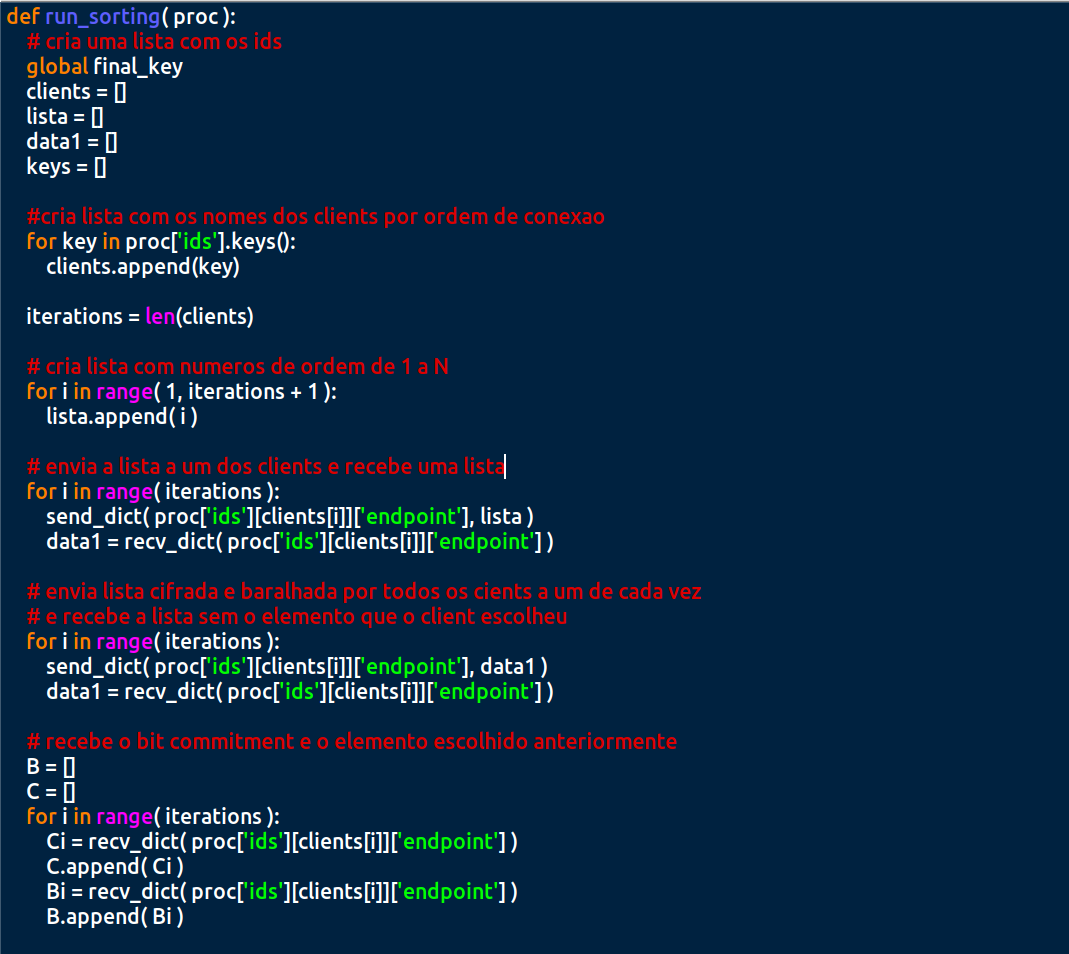
\includegraphics[width=1\linewidth]{RunSorting.png}
  \caption{}
\end{subfigure}%
\begin{subfigure}{.5\textwidth}
  \centering
  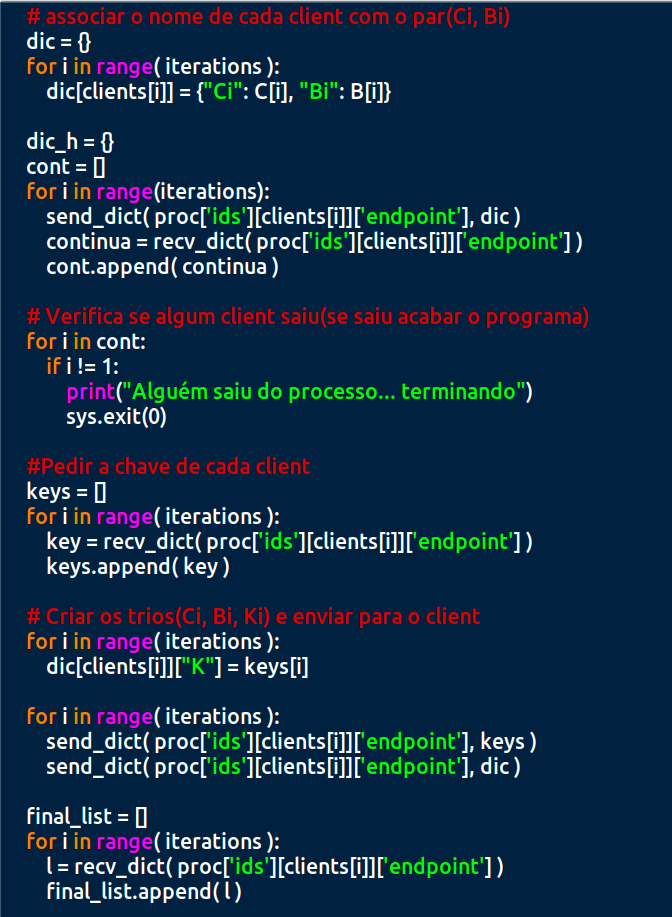
\includegraphics[width=0.9\linewidth]{RunSorting2.png}
  \caption{}
\end{subfigure}
\begin{subfigure}{.5\textwidth}
  \centering
  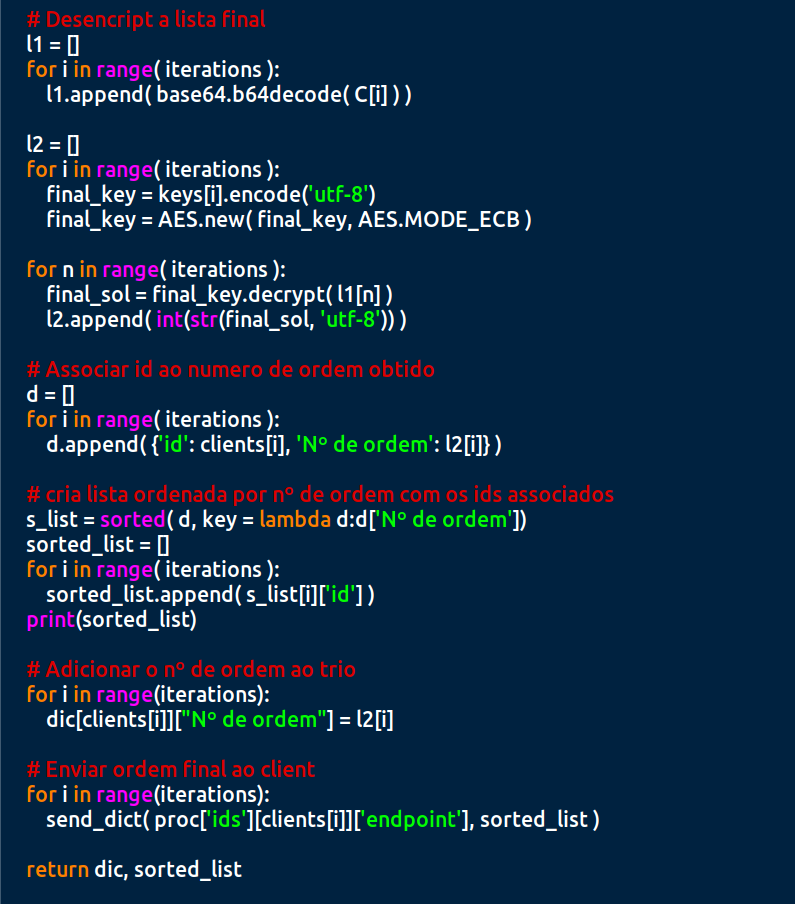
\includegraphics[width=0.9\linewidth]{RunSorting3.png}
  \caption{}
\end{subfigure}%
	\caption{Código de Sorting explicado}
\end{figure}
\paragraph{}
\newpage
\paragraph{}
\paragraph{}
\paragraph{}
\paragraph{}
No que toca à parte encriptar , baralhar e distribuir o nºde ordem pelos participantes foi usada a "def client" do cliente.

\begin{figure}[hbt!]
\centering
\begin{subfigure}{.5\textwidth}
  \centering
  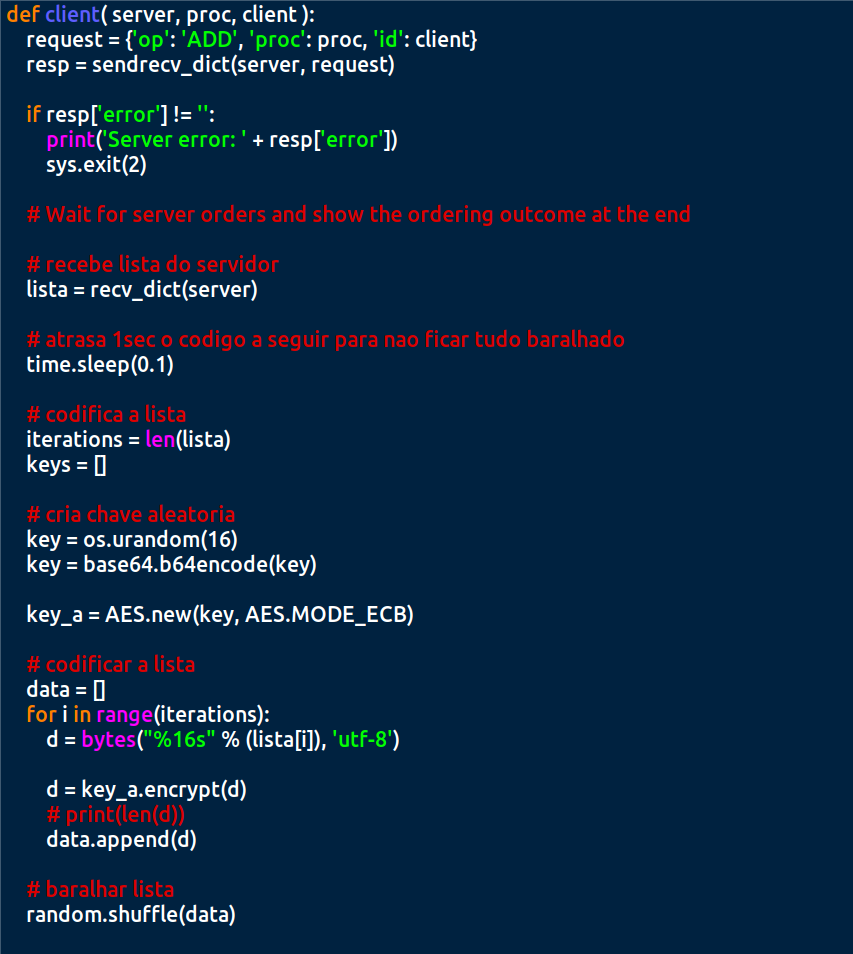
\includegraphics[width=0.9\linewidth]{defClient1.png}
  \caption{}
\end{subfigure}%
\begin{subfigure}{.5\textwidth}
  \centering
  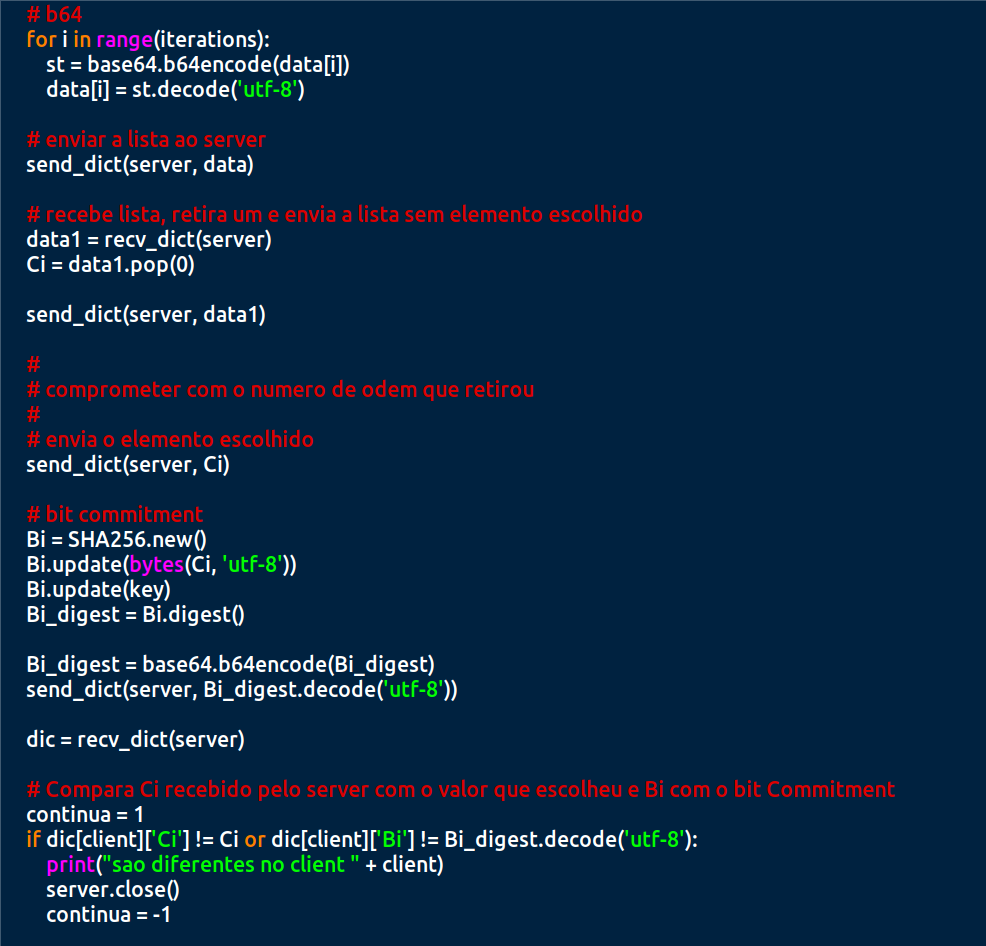
\includegraphics[width=0.9\linewidth]{defClient2.png}
  \caption{}
\end{subfigure}
\begin{subfigure}{.5\textwidth}
  \centering
  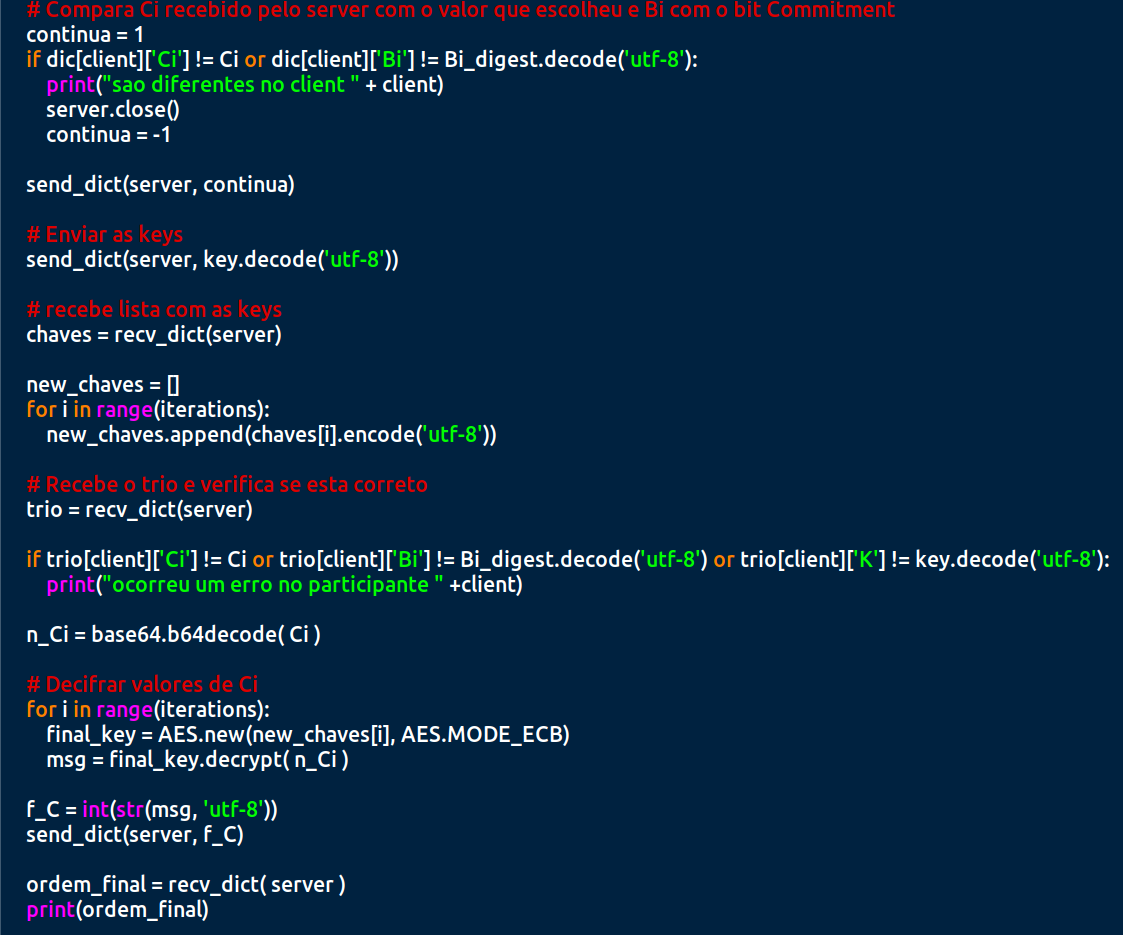
\includegraphics[width=0.9\linewidth]{defClient3.png}
  \caption{}
\end{subfigure}%
	\caption{Código "def client" explicado.}
\end{figure}
\pagebreak
\paragraph{}
\paragraph{}
\paragraph{}

\subsection{Exportação dos dados}
No fim do processo de sorting todos os dados gerados (tais como o nº de ordem, key, bit commitment,o elemento cifrado) de cada um dos participantes devem ser exportados para um ficheiro csv(report.csv).
\begin{figure}[hbt!]
  \centering
  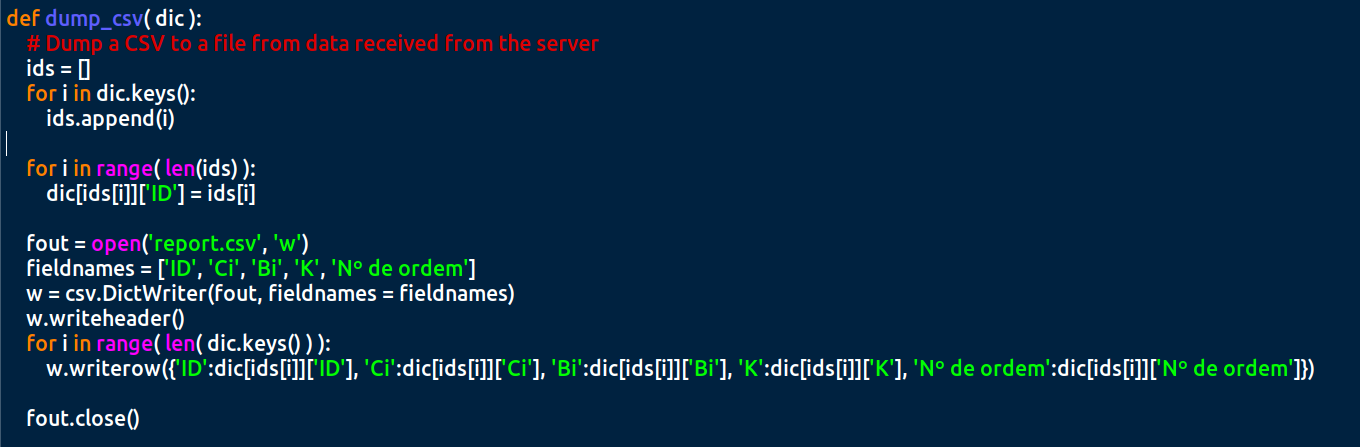
\includegraphics[width=0.9\linewidth]{dumpCSVclient.png}
  \caption{dump\_proc - servidor.}
\end{figure}

\begin{figure}[hbt!]
  \centering
  
\includegraphics[width=0.9\linewidth]{dumpProcServer.png}
  \caption{dump\_csv - cliente.}
\end{figure}
Se admitir-mos que entraram no processo 10 participantes, o resultado do ficheiro CSV final será o seguinte:
\begin{figure}[hbt!]
  \centering
  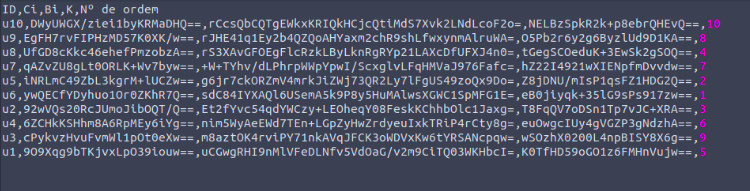
\includegraphics[width=1\linewidth]{CSV.png}
  \caption{report.csv}
\end{figure}

\chapter*{Contribuições dos autores}
Consideramos que houve uma contribuição de 50\% para cada um dos dois membros do grupo

%%%%%%%%%%%%%%%%%%%%%%%%%%%%%%%%%

\printbibliography

\end{document}
